\documentclass[a4paper, 12pt]{article}
\usepackage[total={17cm,25cm}, top=2.5cm, left=2.5cm, right=2.5cm,  includefoot]{geometry}
\usepackage[utf8]{inputenc}
\usepackage{array}
\usepackage{multirow}
\usepackage{hhline}
\usepackage{gensymb}
\usepackage{graphicx}
\graphicspath{ {} }
\usepackage[czech]{babel}
\usepackage{enumitem}
\usepackage{pdfpages}
\usepackage{amsmath}
\usepackage{verbatim}
\usepackage{listings}
\usepackage{hyperref}
\usepackage{amssymb}


\pagestyle{empty} % vypne číslování stránek




\usepackage[OT2,OT1]{fontenc}
\newcommand\cyr
{
\renewcommand\rmdefault{wncyr}
\renewcommand\sfdefault{wncyss}
\renewcommand\encodingdefault{OT2}
\normalfont
\selectfont
}
\DeclareTextFontCommand{\textcyr}{\cyr}
\def\cprime{\char"7E }
\def\cdprime{\char"7F }
\def\eoborotnoye{\char’013}
\def\Eoborotnoye{\char’003}


\begin{document}



\begin{titlepage}
\begin{center}
\noindent
\Large \textbf{České vysoké učení technické v Praze }\\ Fakulta stavební
\vspace{5cm}

\huge

%vložení loga cvut
\begin{figure}[h!]
	\centering
	
\includegraphics[width=7cm]{pictures/logo.png}
\end{figure}

\vspace{0.5cm}

Algoritmy v digitální kartografii \\

\vspace{3cm}

\Huge  
Digitální model terénu a jeho analýzy\\

\vspace{2cm}

\Large
Bc. Petra Pasovská \\
Bc. David Zahradník \\

\end{center}

\end{titlepage}




\pagestyle{plain}     % zapne obyčejné číslování
\setcounter{page}{1}  % nastaví čítač stránek znovu od jedné

\tableofcontents
\newpage

\section{Zadání}
Níže uvedené zadání je kopie ze stránek předmětu. 

\begin{figure}[h!]
	\centering
	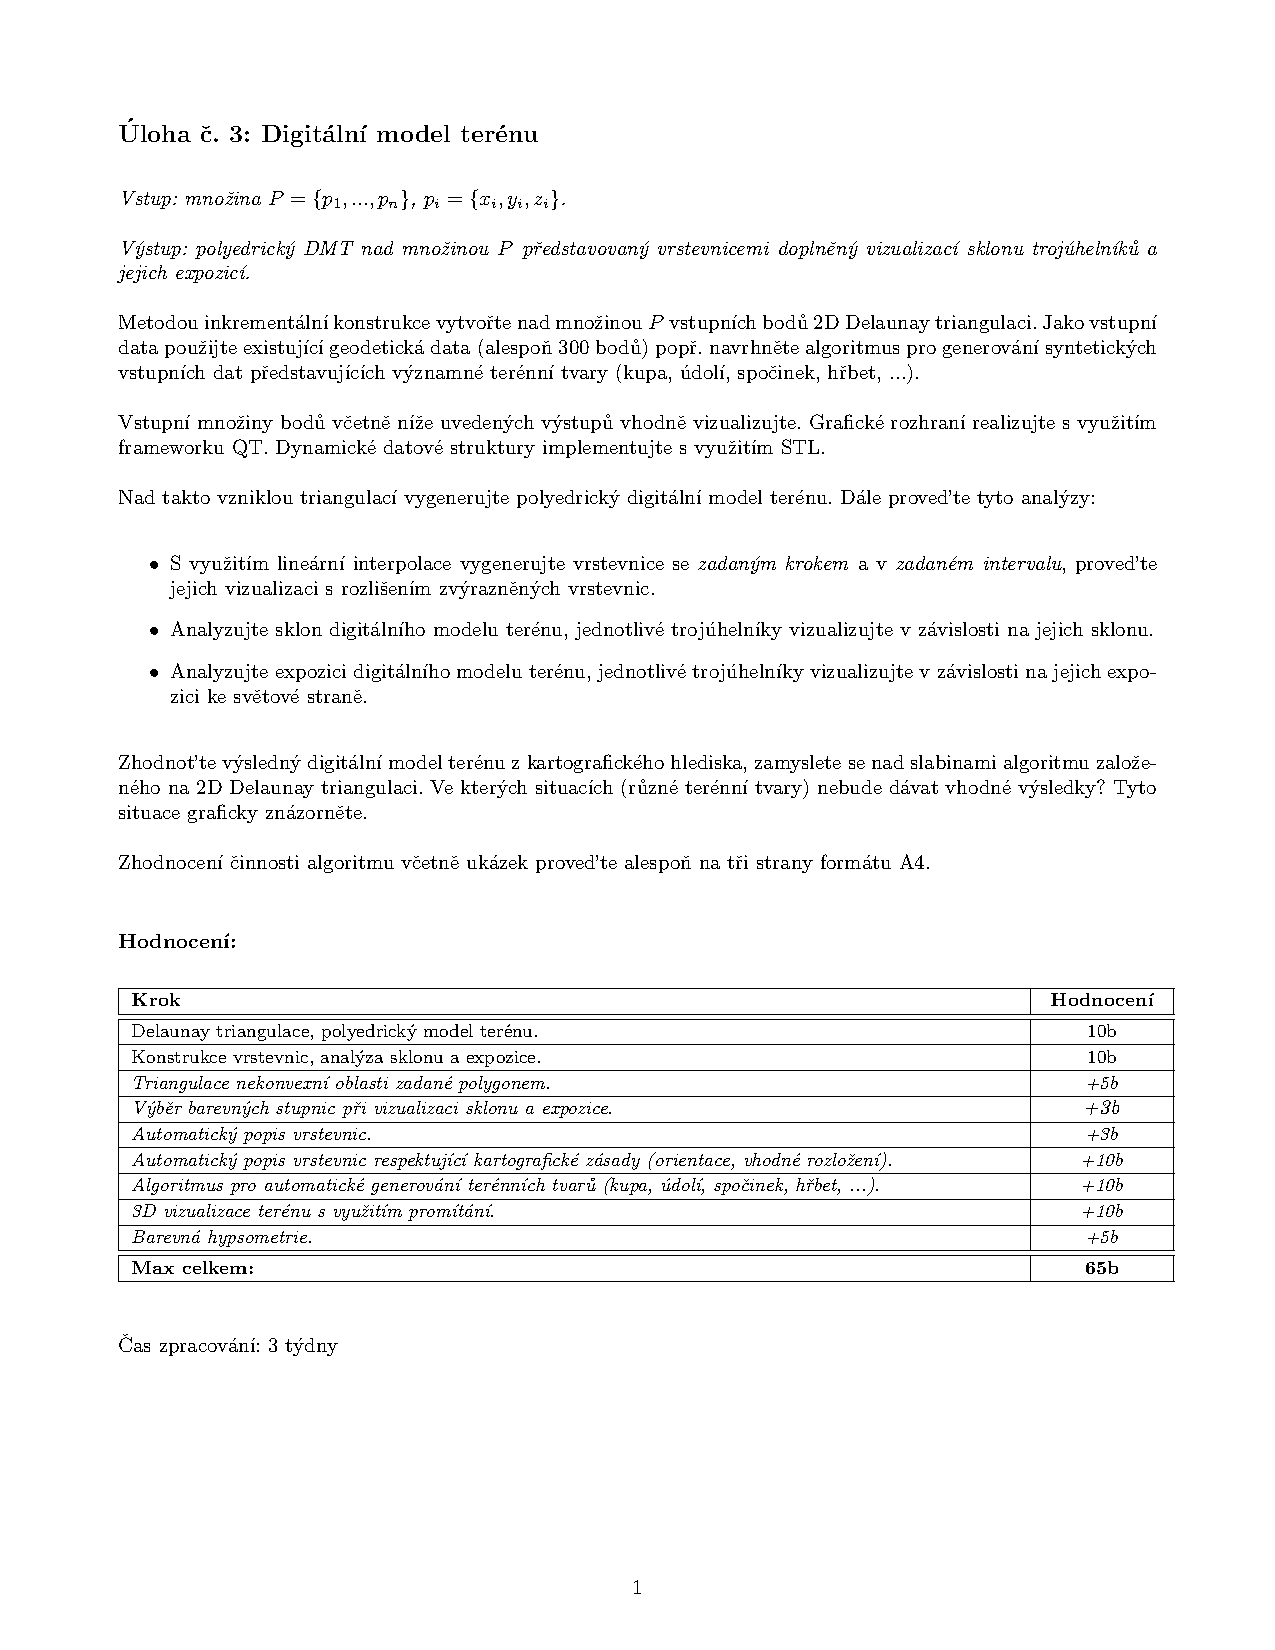
\includegraphics[clip, trim=0cm 5cm 0cm 0cm, width=1.2\textwidth]{zadani.pdf}
\end{figure}

\subsection{Údaje o bonusových úlohách}
Nebyly vytvořeny žádné bonusové úlohy.



\section{Popis a rozbor problému}
Hlavním cílem této úlohy je tvorba aplikace, která nad výškopisnými body vytvoří Delaunay triangulaci, vrstevnice a vypočte sklon a expozici k světovým stranám.\\
\\
Obecně triangulační algoritmy jsou nejvíce zkoumané algoritmy digitální kartografie v dnešní době. Slouží k různým účelům např. tvorba digitálního modelu terénu, plánování pohybu robotů, detekce otisků prstů.  [Zdroj: 1]
\\
Při triangulaci je kladen důraz na to, aby vytvořené trojúhelníky byly pokud možno rovnostranné. V případě, že takovéto trojúhelníky sestavíme, každý z vytvořených trojúhelníků musí co nejlépe reprezentovat hodnotu povrchu. Zároveň je nutné, aby byla produkována jednoznačná triangulace nezávisle na počátečním bodě či na orientaci množiny bodů. Delaunayho triangulace tyto podmínky obecně splňuje, přesto existují výjimky, kdy nemá Delaunayho triangulace jednoznačné řešení. Tento stav může nastat pro určité množiny dat, např. pravoúhlý grid. [Zdroj: 2]\\
\\
Delaunayho triangulace je velmi podobná Dirichletově teselaci, která rozdělí body unikátní množinou polygonů, které jsou označovány jako Thiessenovy polygony či Voronoiovy diagramy. Voronoiovy diagramy jsou takové polygony, které vytvoří kolem všech bodů takové oblasti, že všechna místa uvnitř leží nejblíže k danému bodu. \\
\\
Voronoiovy diagramy mají v dnešní době řadu využití. V meteorologii se využívají pro určení množství srážek v daném území, v astronomii pro studium galaxií, v molekulární biologii pro hledání tunelů v molekulách, v geografii pro sledování osídlení či pro plánování cest při pohybu robotů. Voroniovy diagramy se vyskytují i v přírodě, můžeme je nalézt na kůži žirafy, na krunýři želvy, na povrchu pouště Atacamy či na křídle vážky. [Zdroj: 3]

\begin{figure}[h!]
\centering
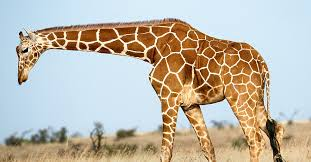
\includegraphics[width=5cm]{pictures/zirafa.jpg}
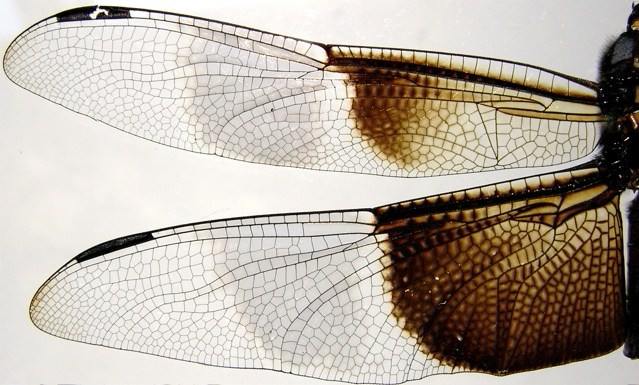
\includegraphics[width=5cm]{pictures/vazka.jpg}
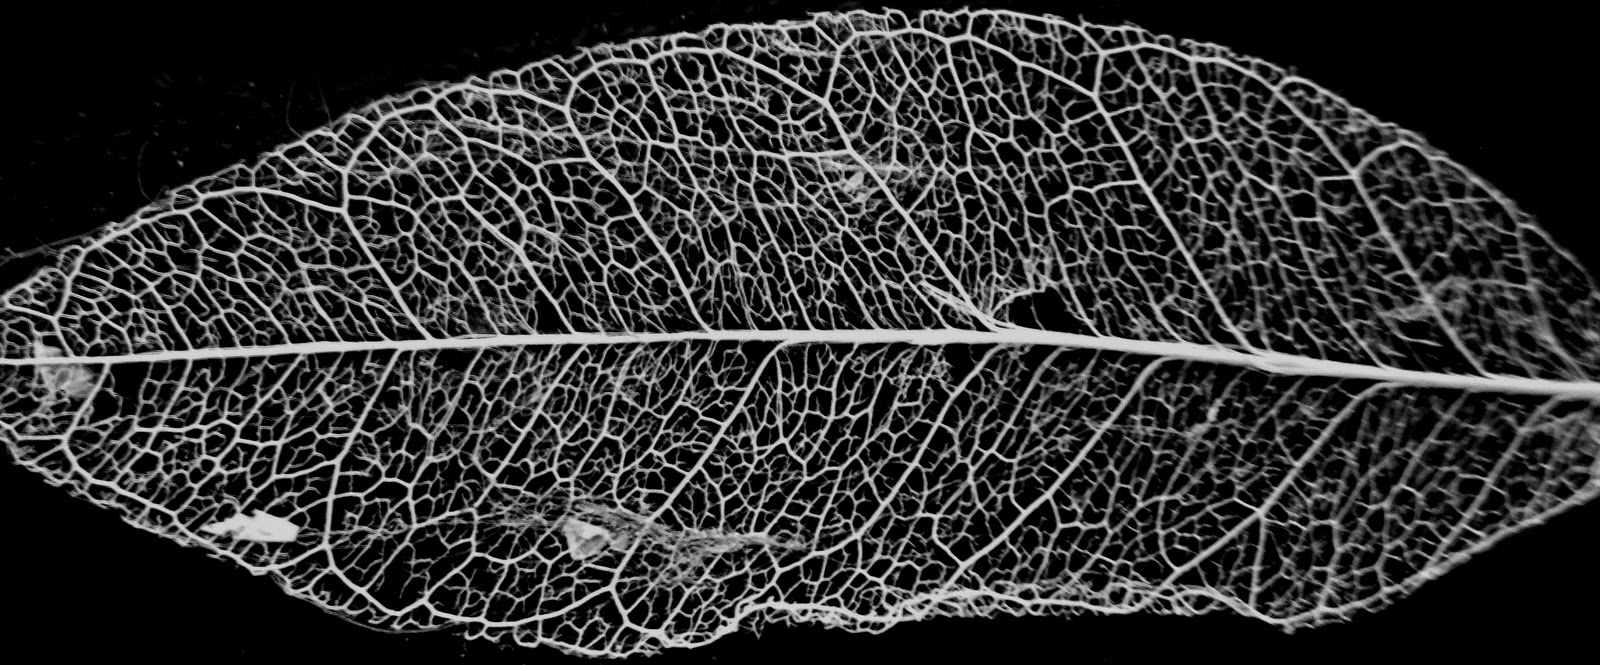
\includegraphics[width=5cm]{pictures/list.jpg}
\caption{Voronoiovy diagramy v přírodě - na kůži žirafy, na křídle vážky a na žilkování listu}
\end{figure}


Tato dokumentace je však zaměřena na triangulaci. Existuje mnoho druhů triangulace v závislosti na geometrické konstrukci - Greedy triangulace, Minimum Weight Triangulation, Constrained triangulation, nejčastěji používaná je však Delaunayho triangulace.  Zjednodušeně si lze Delaunyho triangulaci představit tak, že zvolíme tři body, kterým opíšeme kružnici. Pokud uvnitř kružnice neleží žádný další bod, vytvoři se trojúhelník. Pokud se uvnitř bod nachází, zvolí se jiné tři body. Tato triangulace je jednoznačná, pokud žádné čtyři body neleží na kružnici. Trojúhelníky vzniklé Delaunyho triangulací se nejvíce blíží rovnostranným trojúhelníkům. \\
\\
V dnešní době se kromě analýzy prostorových dat využívá Delaunyho triangulace a Voronoiovy diagramy například v grafice. Takto vytvořené obrazy jsou nazývaný Delaunyho rastry (The Delaunay Raster). Autoři takovýchto děl jsou schopni pomocí Delaunyho triangulace sami vytvářet obrazy, případně převést existující obraz na triangulaci. [Zdroj: 4]

\begin{figure}[h!]
\centering
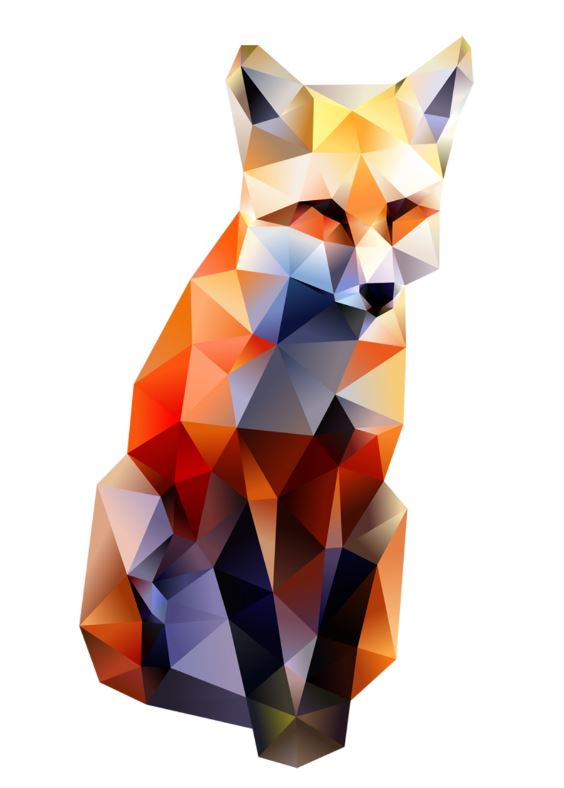
\includegraphics[width=5cm]{pictures/liska.jpg}
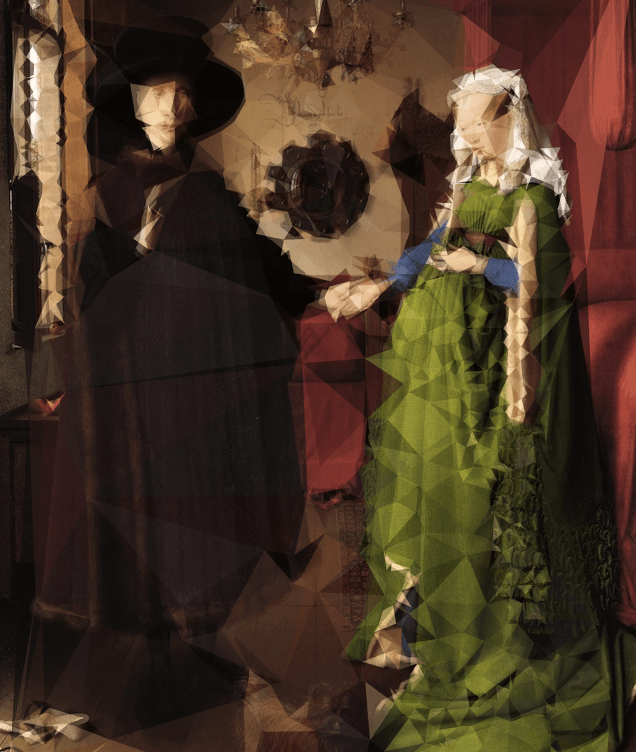
\includegraphics[width=5cm]{pictures/jan_van_eyck.png}
\caption{Použití Delaunyho triangulace v grafice - na vytvořeném novém obrázku lišky a na přepracování obrazu od Jana van Eycka}
\end{figure}

\section{Popis použitých algoritmů}
Existuje několik způsobů jak vytvořit triangulaci s různými kritérii. V této úloze jsme se zabývali Delaunayho triangulací pomocí metody inkrementální konstrukce.

\subsection{Delaunayho triangulace}
Delaunayho triangulace je nejčastěji používanou triangulací při tvorbě digitálního modelu terénu. Delaunayho triagulaci lze provádět v rovině i v prostoru.
\\
\subsubsection{Vlastnosti}

\begin{enumerate}
\item Uvnitř opsané kružnice libovolného trojúhelníku triangulace neleží žádný jiný bod.
\item Maximalizuje minimální úhel, avšak neminimalizuje maximální úhel v trojúhelníku.
\item Vůči kritériu minimálního úhlu je lokálně i globálně optimální.
\item Triangulace je jednoznačná, pokud čtyři body neleží na kružnici.
\end{enumerate}


Triangulace byla realizována pomocí metody inkrementální konstrukce. Tento algoritmus je založen na postupném hledání bodu, který k bodům hrany tvoří minimální opsanou kružnici. Každá hrana je orientovaná a bod se hledá pouze v její levé polorovině.\\
\\
Je-li nalezen bod s výše uvedeným kritériem, vytvoří se dvě nové hrany, které jsou přidány do triangulace. Nenalezne-li se daný bod, prohodí se orientace hrany a hledání pokračuje.\\
\\
Hrany, které nebyly zlegalizovány (nebyl k nim ještě nalezen třetí bod), jsou ukládány do struktury Active Edge List (AEL). Pokud k dané hraně byl nalezen třetí bod, hrana se ze struktury odstraní. Než je hrana vložena do struktury, kontroluje se, zda hrana už ve struktuře není s opačnou orientací. Pokud je, hrana se nevloží. Algoritmus probíhá do té doby, dokud není struktura AEL prázdná.

\subsubsection{Implementace metody}
\begin{enumerate}
\item Nalezení pivota q a k němu nejbližší bod:  $ q = min(y_i) $ 
\item Hledání prvního Delaunayho bodu.
\item Vytvoření prvního Delaunay trojúhelníku.
\item Hrany trojúhelníka se uloží do triangulace a do AEL.
\item Dokud není AEL prázdný proveď.
\subitem Hledej Delaunay bod k hraně z AEL.
\subitem Pokud Delaunay bod existuje.
\subsubitem Přidej nové hrany do DT.
\subsubitem Pokud nová hrana není v AEL přidej.
\end{enumerate}

\subsection{Vrstevnice}
V úloze byly vrstevnice konstruovány lineární interpolací. U lineární interpolace je rozestup vrstevnice mezi dvěma body konstantní, tedy i spád. Při konstrukci vrstevnic hledáme průsečnici vodorovné roviny o výšce Z a rovinu trojúhelníka triangulace.\\

\subsubsection{Implementace metody}
\begin{enumerate}
\item Pro všechny hrany triangulace:
\subitem Otestuj zda hrana protíná vodorovnou rovinu o výšce Z:
\subitem Pokud protíná spočti polohové souřadnice.
\subitem Vytvoř hranu tvořící vrstevnici.

\end{enumerate}

\subsection{Sklon terénu}
Skon terénu je definován jako úhel mezi normálovým vektorem (0,0,1) a normálovým vektorem roviny trojúhelníku.

\subsubsection{Implementace metody}
\begin{enumerate}
\item Pro všechny trojúhelníky triangulace:
\subitem Vypočti sklon:
\end{enumerate}

\subsection{Expozice terénu}
Expozice terénu je definována jako azimut k průmětu normálového vektoru roviny trojúhelníku do roviny x,y.

\subsubsection{Implementace metody}
\begin{enumerate}
\item Pro všechny trojúhelníky triangulace:
\subitem Vypočti expozici:
\end{enumerate}

\section{Informace o bonusových úlohách}


\section{Vstupní data}
V aplikaci lze bud generovat jednoduchá data, nebo je lze importovat ve formátu .txt\\

Vzor vstupních dat ve formátu .txt\\
 748720.120    1048636.300     306.100\\
 748720.750    1048636.130     305.940\\
 748721.600    1048635.700     306.080\\
 748721.610    1048628.180     305.570\\

\section{Výstupní data}

\section{Aplikace}


\section{Dokumentace}
\subsection{Třídy}
\subsubsection{Algorithms}
Třída Algorithms obsahuje několik metod. Metody jsou určeny pro výpočty použitých algoritmů.
\\

\textbf{double distance(QPoint3D p1, QPoint3D p2)}\\
Metoda, jejíž návratová hodnota je typu double, vrací velikost spojnice mezi dvěma body.
\\

\textbf{TPosition getPointLinePosition(QPoint \&q, QPoint \&a, QPoint \&b)}\\
Tato metoda slouží k určení pozice bodu q vůči linii tvořené body a, b. Výstupem metody je LEFT, RIGHT nebo ON.\\

\textbf{double getCircleRadius(QPoint3D \&p1, QPoint3D \&p2, QPoint3D \&p3, QPoint3D \&c)}\\
Metoda jejíž návratová hodnota je typu double, vrací velikost poloměru kružnice tvořené třemi vstupními body.\\

\textbf{int getNearestPoint(QPoint3D \&p, std::vector\textless QPoint3D\textgreater \&points)}\\
Tato metoda slouží k nalezení indexu nejbližšího bodu k bodu p.\\

\textbf{int getDelaunayPoint(QPoint3D \&s, QPoint3D \&e, std::vector\textless QPoint3D \textgreater \&points)}\\
Tato metoda slouží k nalezení indexu bodu, který splňuje Delaunayho vlastnosti.\\

\textbf{std::vector\textless Edge \textgreater DT(std::vector \textless QPoint3D \textgreater \&points)}\\
Metoda vytváří nad vektorem bodů Delaunayho triangulaci, která je reprezentována jako vektor hran.\\

\textbf{QPoint3D getContourPoint(QPoint3D \&p1, QPoint3D \&p2, double z)}\\
Metoda vypočte průsečík hrany, tvořenou 3D body p1 a p2, a rovinou definovanou Z souřadnicí.\\

\textbf{std::vector\textless Edge \textgreater createContours(std::vector\textless Edge \textgreater \&dt, $double z_min, double z_max, double dz$)}\\
Metoda z triangulace dt v zadaném intervalu v ose Z $<z_{min} ; z_{max}>$ s intervalem vrstevnic dz vrátí vektor hran definující vrstevnice.\\

\textbf{double getSlope(QPoint3D \&p1, QPoint3D \&p2, QPoint3D \&p3)}\\
Tato metoda slouží k vypočetní hodnoty sklonu trojúhelníku definovanému 3D body p1, p2 a p3.\\

\textbf{double getAspect(QPoint3D \&p1, QPoint3D \&p2, QPoint3D \&p3)}\\
Tato metoda slouží k vypočetní hodnoty expozice trojúhelníku definovanému 3D body p1, p2 a p3.\\

\textbf{std::vector\textless Triangle\textgreater analyzeDTM(std::vector\textless Edge \textgreater \&dt)}\\
\\

\textbf{std::vector\textless QPoint3D\textgreater generateHill()}\\
\\

\textbf{std::vector\textless QPoint3D\textgreater generateValley())}\\
\\

\textbf{std::vector\textless QPoint3D\textgreater generateMountains()}\\
\\

\textbf{std::vector\textless QPoint3D\textgreater generateRest())}\\
\\

\subsubsection{Draw}
Třída Draw obsahuje několik metod. Metody jsou určeny pro generování a vykreslování proměných.
\\

\textbf{void paintEvent(QPaintEvent *e)}\\
Metoda slouží k vykreslení vytvořených, generovaných bodů a zobrazení výsledků použitých algoritmů.
\\

\textbf{void mousePressEvent(QMouseEvent *e)}\\
Metoda uloží bod se souřadnicemi místa kliknutí v zobrazovacím okně.
\\

\textbf{void clearDT()}\\
Metoda slouží k vymazání proměnných a k překreslení
\\

\textbf{void clearPoints()}\\
Metoda slouží k vymazání bodů.
\\

\textbf{void setPoints(std::vector\textless QPoint3D \textgreater points\_)}\\
Metoda slouží pro převod bodů do vykreslovacího okna.\\

\textbf{std::vector\textless QPoint3D \textgreater \& getPoints()}\\
Metoda slouží pro převod bodů z vykreslovacího okna.\\

\textbf{std::vector\textless Edge \textgreater \& getDT()}\\
Metoda slouží pro převod Delaunayho triangulace z vykreslovacího okna.\\

\textbf{void setDT(std::vector\textless Edge\textgreater \&dt\_)}\\
Metoda slouží pro převod Delaunayho triangulace do vykreslovacího okna.\\

\textbf{void setContours(std::vector\textless Edge\textgreater\&contours\_)}\\
Metoda slouží pro převod vrtevnic do vykreslovacího okna.\\

\textbf{void setDTM(std::vector\textless Triangle\textgreater \&dtm\_)}\\
Metoda slouží pro převod trojúhelníku triangulace a jeho informací o sklonu a expozici terénu\\

\textbf{void importPolygons(std::string \&path, std::vector\textless QPoint3D \textgreater \&points,  QSizeF \&canvas\_size, double \&min\_z, double \&max\_z)}\\
Metoda slouží pro import vrstevnic, z cesty path naplní vektor points body a uloží hodnotu s minimální a maximální souřadnicí. Proměnná canvas\_size slouží k vykreslení v rozsahu importovaných dat.\\

\textbf{void setSlope(bool slope\_)}\\
Metoda slouží jako podmínka TRUE/FALSE pro vykreslení sklonu terénu.\\

\textbf{void setAspect(bool aspect\_)}\\
Metoda slouží jako podmínka TRUE/FALSE pro vykreslení expozice terénu.\\



\subsubsection{SortByXAsc}
Třída SortByXAsc slouží k porovnání souřadnic v ose x.\\


\textbf{bool operator()(QPoint \&p1, QPoint \&p2)}\\
Přetížený operátor () vrátí bod s větší souřadnicí x z dvojice bodů.\\

\subsubsection{Edge}
\textbf{Edge(QPoint3D \&start, QPoint3D \&end)}\\
Třída Edge je konstruována ze dvou 3D bodů, počátek a konec hrany. Třída slouží k uložení hrany triangulace a nebo vrstevnic.\\
    
\textbf{QPoint3D \&getS()}\\
Metoda vrátí počáteční bod hrany.\\

\textbf{QPoint3D \& getE()}\\
Metoda vrátí koncový bod hrany.\\

\textbf{void switchOr()}\\
Metoda prohodí orientaci hrany.\\

\subsubsection{QPoint3D}
\textbf{QPoint3D(double x, double y, double z\_)}\\
Třída QPoint3D je odvozena z třídy QPointF a složí k uložení bodu s informací o výšce.\\

\textbf{double getZ()}\\
Metoda vrátí výšku bodu.\\

\textbf{void setZ(double z\_)}\\
Metoda nastaví výšku bodu.\\

\subsubsection{Triangle}
\textbf{Triangle(QPoint3D \&p1\_, QPoint3D \&p2\_, QPoint3D \&p3\_, double slope\_, double aspect\_))}\\
Třída QPoint3D složí k uložení trojúhelníku definovaného body p1, p2, p3 a jeho informaci o sklonu a expozici.\\

\textbf{ QPoint3D getP1()}\\
Metoda vrátí první bod trojúhelníku.\\

\textbf{ QPoint3D getP2()}\\
Metoda vrátí druhý bod trojúhelníku.\\

\textbf{ QPoint3D getP3()}\\
Metoda vrátí třetí bod trojúhelníku.\\

\textbf{double getSlope()}\\
Metoda vrátí sklon trojúhelníku.\\

\textbf{double getAspect()}\\
Metoda vrátí expozici trojúhelníku.\\

\subsubsection{Widget}

\textbf{void on\_pushButton\_clicked()}\\
Při stisknutí tlačítka Denaulay se zavolá metoda třídy Algorithms DT a výsledek se zobrazí v okně.
\\

\textbf{void on\_pushButton\_3\_clicked()}\\
Při stisknutí tlačítka Clear se zavolá metoda třídy Draw clearDT.
\\

\textbf{void on\_pushButton\_2\_clicked()}\\
Při stisknutí tlačítka Create Contours se zavolá metoda třídy Algorithms createContours a výsledek se zobrazí v okně.
\\

\textbf{void on\_pushButton\_4\_clicked()}\\
Při stisknutí tlačítka AnalyzeDTM se zavolá metoda třídy Algorithms analyzeDTM a výsledek se zobrazí v okně.
\\

\textbf{void on\_pushButton\_5\_clicked()}\\
Při stisknutí tlačítka Generate a výběru z comboboxu se vygenerují body terénu.
\\

\textbf{void on\_pushButton\_6\_clicked()}\\
Při stisknutí tlačítka Import, se otevře okno pro výběr importovaných dat.
\\



\clearpage
\section{Závěr}
Byla vytvořena aplikace, která nad importovanými body vytvoří Delaunayho triangulaci, vykreslí vrstevnice, sklon a expozici terénu. Aplikace má nějaké nedostatky, které autoři nestihli opravit.\\

\subsection{Delaunayho triangulace}
Vzhledem k implementaci triangulace pro výběr trojúhelníku s vyhledáním nejmenší opsané kružnice, algoritmus selhává pro body na mřížce. Triangulace je pro tyto body nejednoznačná a další výpočty selhávají. Obecně se ví, že Delaunyho triangulace nemá pro body na mřížce jednoznačné řešení. Tento problém by se mohl vyřešit vložením povinných hran.\\

V aplikaci bohužel nelze nadefinovat povinné hrany, které jsou důležité pro terénní tvary, například pro terénní hranu či propast. Proto algoritmus není použitelný pro data s těmito typy terénních tvarů. Důvod je zřejmý z implementace triangulace.\\

V aplikaci též nelze nastavit zájmovou oblast, proto je nutné před výpočtem algoritmu odstranit body, nad kterými nechceme provádět triangulaci.\\

Aplikace je užitečná pro výškopisná data v terénu bez povinných hran a kde data nepotřebují být upravována, viz předchozí odstavec. \\

\subsection{Vrstevnice}
Pro vykreslení vrstevnic byla použita lineární interpolace, která má svoje úskalí. Jelikož pro výpočet vrstevnic není řešené vyhlazení vrstevnic, výsledek není vhodný ke chlubení. Pro kvalitní výsledek by bylo vhodnější použít morfologickou interpolaci, která předpokládá plynulou změnu spádu terénu mezi jednotlivými body. Není pro ni však definován žádný exaktní postup, tudíž nelze naimplementovat. \\

Autoři neřešili vykreslení hlavní vrstevnice zesílenou čárou ani popis vrstevnic. \\

\subsection{Sklon a expozice terénu}
Při výpočtu sklonu a expozice terénu vzniká problém v rovinatém území. Při výpočtu vznikají zaokrouhlovací chyby, které se promítnou do sklonu a expozice. Proto se terén jeví uživateli nerovinný.\\

Do aplikace by se hodila legenda expozice terénu.\\

\section{Náměty na vylepšení}
V aplikaci by se dalo vylepšit zobrazení vrstevnic, mohla by být zvýrazněná zesílená vrstevnice a zobrazen popis vrstevnic. 
V aplikaci by mohla být možnost exportu jak triangulace tak vrstevnic. 
V aplikaci mi mohlo být řešeno odstranění naimportovaných bodů, nad kterými uživatel nechce počítat triangulaci. 
V aplikaci by mohla být volba pro uživatele nastavení výpočet vrstevnic v určitém rozsahu nadmořské výšky.\\


\clearpage
\section{Reference}

\begin{enumerate}
\item  BAYER, Tomáš. Geometrické vyhledávání [online][cit. 1. 12.2018]. \\
Dostupné z: https://web.natur.cuni.cz/~bayertom/images/courses/Adk/adk5.pdf  \\

\item JANEČKA, Karel, PACINA, Jan. Výukové materiály k předmětu KMA/UGI - Západočeská univerzita v Plzni. [online][cit. 4. 12. 2018]\\
Dostupné z: https://kgm.zcu.cz/studium/ugi/cviceni/ch08s01.html\\

\item BENEŠ, Petr. Diplomová práce: Voroného diagramy v molekulární chemii. [online] [cit. 4. 12. 2018]\\
Dostupné z: https://is.muni.cz/th/m1tcs/benes\_dp.pdf \\

\item PUCKEY, Jonathan. Delaunay Raster. [online] [cit. 4. 12. 2018]\\
Dostupné z: https://jonathanpuckey.com/projects/delaunay-raster/index.html





\end{enumerate}
\end{document}



 